\chapter{Singularity Analysis}
\label{ch04:top}

Chapter~2 showed how the radius of convergence captures the exponential scale of a coefficient sequence. This chapter adds the next level of information. Under suitable analyticity hypotheses, the \emph{local form} of a generating function near its dominant singularity determines the polynomial correction to that exponential growth. That principle is the content of the Flajolet--Odlyzko transfer theorem \cite{FlajoletOdlyzko1990}.

This chapter has two different goals. First, it explains the main theorem and the shape of its hypotheses. Second, it works through the most important model cases so the theorem does not feel like a black box dropped from the sky. What it does \emph{not} do is give a beginner-friendly full proof of the transfer theorem; the complex-analytic proof uses more contour machinery than we want to develop here. Whenever we are only giving the roadmap, I will say so explicitly.

\section{Exponential Growth Rate Revisited}

Let
\[
  A(z) = \sum_{n \ge 0} a_n z^n
\]
have radius of convergence $\rho$. By Cauchy--Hadamard,
\[
  \limsup_{n \to \infty} |a_n|^{1/n} = \rho^{-1}.
\]
So for every $\varepsilon > 0$, eventually
\[
  |a_n|^{1/n} \le \rho^{-1} + \varepsilon,
\]
and therefore
\[
  |a_n| \le (\rho^{-1}+\varepsilon)^n
\]
for all sufficiently large $n$. In this sense, $\rho^{-n}$ is the correct exponential scale.

What the radius does \emph{not} determine is the subexponential correction. For example,
\[
  n^{1/2}\rho^{-n}
  \qquad\text{and}\qquad
  n^{-3/2}\rho^{-n}
\]
have the same exponential part because
\[
  \lim_{n \to \infty} (n^{1/2})^{1/n} = \lim_{n \to \infty} (n^{-3/2})^{1/n} = 1.
\]
The difference between those two sequences lies entirely in the polynomial prefactor. Singularity analysis is what recovers that finer information.

\section{Dominant Singularities and Periodicity}

\begin{definition}
Assume $A(z)$ has finite radius of convergence $\rho < \infty$. A \emph{dominant singularity} of $A$ is a point $\zeta$ with $|\zeta|=\rho$ such that the holomorphic function represented by the power series on $|z|<\rho$ cannot be analytically continued through $\zeta$.
\end{definition}

The phrase ``cannot be continued through $\zeta$'' means that no holomorphic extension exists on any neighborhood of $\zeta$ that agrees with the original power series on the part of that neighborhood lying inside the disk of convergence.

There may be more than one dominant singularity. The simplest example is
\[
  \frac{1}{1-z^2} = \frac{1}{2}\left(\frac{1}{1-z} + \frac{1}{1+z}\right).
\]
Its radius of convergence is $1$, and the dominant singularities are $z=1$ and $z=-1$. The coefficient of $z^n$ is
\[
  \frac{1}{2}(1+(-1)^n),
\]
so the second singularity contributes the alternating factor $(-1)^n = (-1)^{-n}$. This is why multiple dominant singularities can produce oscillation instead of a clean single-term asymptotic.

To keep the main theorem readable, it is common to restrict first to the \emph{aperiodic} case.

\begin{definition}
A coefficient sequence $(a_n)$ is \emph{aperiodic} if
\[
  \gcd\{n \ge 0 : a_n \ne 0\} = 1.
\]
If the gcd is $d>1$, then all nonzero coefficients lie on a lattice of step $d$, and one typically expects $d$ different dominant singularities related by roots of unity.
\end{definition}

In many positive combinatorial classes, aperiodicity is the condition that rules out forced periodic oscillation. For the rest of the chapter, we focus on the cleanest situation: a unique dominant singularity at a positive real point $z=\rho$.

\section{Rational Generating Functions as a Prototype}

The rational case can be understood exactly, and it provides the first model for the general theorem.

\begin{proposition}
For every integer $m \ge 1$,
\[
  \frac{1}{(1-z/\rho)^m} = \sum_{n \ge 0} \binom{n+m-1}{m-1}\rho^{-n} z^n.
\]
Consequently,
\[
  [z^n]\frac{1}{(1-z/\rho)^m} = \binom{n+m-1}{m-1}\rho^{-n}
  \sim \frac{n^{m-1}}{(m-1)!}\rho^{-n}.
\]
\end{proposition}

\begin{proof}
Apply the generalized binomial theorem from Chapter~1 with $\alpha=-m$ and $w=-z/\rho$:
\[
  (1-w)^{-m} = \sum_{n \ge 0} \binom{-m}{n}(-w)^n.
\]
The standard identity
\[
  \binom{-m}{n}(-1)^n = \binom{n+m-1}{m-1}
\]
gives the displayed series.

For the asymptotic, write
\[
  \binom{n+m-1}{m-1} = \frac{(n+m-1)(n+m-2)\cdots(n+1)}{(m-1)!}.
\]
Dividing by $n^{m-1}$ yields
\[
  \frac{\binom{n+m-1}{m-1}}{n^{m-1}}
  = \frac{(1+\frac{m-1}{n})(1+\frac{m-2}{n})\cdots(1+\frac{1}{n})}{(m-1)!}
  \to \frac{1}{(m-1)!}.
\]
So
\[
  \binom{n+m-1}{m-1} \sim \frac{n^{m-1}}{(m-1)!}.
\]
\end{proof}

Now take a general proper rational function $A(z)=P(z)/Q(z)$. Partial fractions express it as a finite sum of terms of the form
\[
  \frac{c_{j,m}}{(1-z/\zeta_j)^m},
\]
where the $\zeta_j$ are the poles of $A$. Each such term contributes a polynomial in $n$ times $\zeta_j^{-n}$. If $\rho$ is the unique pole of smallest modulus, then every other term is exponentially smaller because
\[
  \left|\frac{\rho}{\zeta_j}\right|^n \to 0
  \qquad\text{whenever } |\zeta_j|>\rho.
\]
So the nearest pole determines the asymptotic behavior.

\begin{example}[Fibonacci numbers]
Chapter~1 showed that
\[
  F(z) = \frac{z}{1-z-z^2}
\]
is the generating function of the Fibonacci sequence. Its poles are at
\[
  z = \frac{-1 \pm \sqrt{5}}{2} = \frac{1}{\varphi},\, -\varphi.
\]
The dominant pole is $\rho = 1/\varphi$, and it is simple. The partial fraction formula from Chapter~1 gives
\[
  F(z) = \frac{1/\sqrt{5}}{1-\varphi z} - \frac{1/\sqrt{5}}{1-\hat\varphi z}.
\]
Therefore
\[
  F_n = \frac{\varphi^n - \hat\varphi^n}{\sqrt{5}},
\]
and in particular
\[
  F_n \sim \frac{\varphi^n}{\sqrt{5}}.
\]
Since $|\hat\varphi|=1/\varphi<1$, the second term is exponentially smaller, and for every $n \ge 1$ its absolute value is at most
\[
  \frac{\varphi^{-n}}{\sqrt{5}} \le \frac{1}{\sqrt{5}\,\varphi} < \frac{1}{2}.
\]
\end{example}

\section{The Transfer Theorem}

Rational functions are only the beginning. Catalan numbers, trees, and many recursive combinatorial classes lead to algebraic singularities such as square roots. The general tool is the transfer theorem.

First we need the domain on which the local singular model is valid.

\begin{definition}
For $\rho > 0$, $\phi \in (0,\pi/2)$, and $\eta > \rho$, the \emph{$\Delta$-domain at $\rho$} is
\[
  \Delta(\rho,\phi,\eta) = \{z \in \mathbb{C} : |z|<\eta,\; z \ne \rho,\; |\arg(z-\rho)|>\phi\}.
\]
A function is \emph{$\Delta$-analytic at $\rho$} if it is analytic in some such domain.
\end{definition}

Geometrically, this is a disk of radius $\eta$ centered at the origin with a small wedge removed around the ray starting at $\rho$ and extending to the right. The removed wedge is exactly the place where a branch cut for $(1-z/\rho)^{\alpha}$ is allowed to sit.

\begin{center}
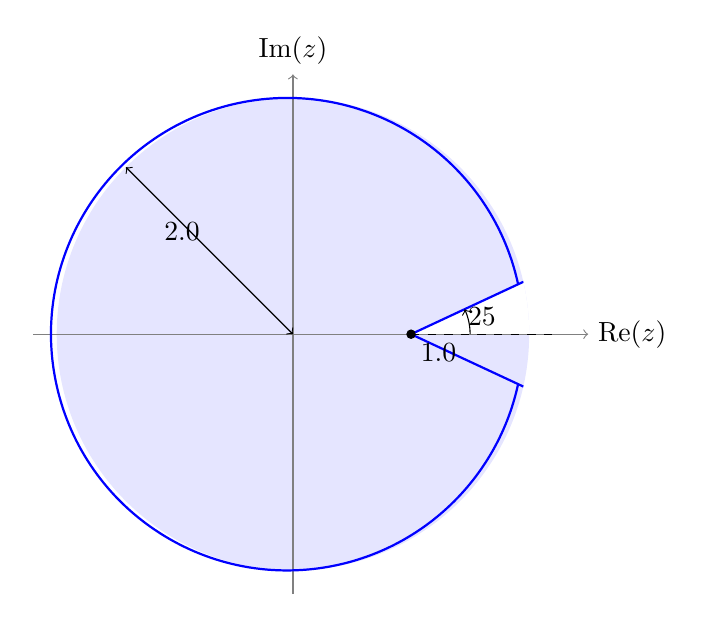
\begin{tikzpicture}[scale=1.5]
  \def\rho{1.0}
  \def\eta{2.0}
  \def\phi{25} % angle in degrees
  
  % Fill the Delta domain
  \begin{scope}
    \clip (0,0) circle (\eta);
    \fill[blue!10] (-2.5,-2.5) rectangle (2.5,2.5);
    \fill[white] (\rho,0) -- ++(\phi:2.5) -- ++(-\phi:2.5) -- cycle;
  \end{scope}

  % Draw axes
  \draw[->, gray] (-2.2, 0) -- (2.5, 0) node[right, text=black] {$\mathrm{Re}(z)$};
  \draw[->, gray] (0, -2.2) -- (0, 2.2) node[above, text=black] {$\mathrm{Im}(z)$};
  
  % Draw the boundary of the Delta domain
  \begin{scope}
    \clip (0,0) circle (\eta);
    \draw[thick, blue] (\rho,0) -- ++(\phi:2.5);
    \draw[thick, blue] (\rho,0) -- ++(-\phi:2.5);
  \end{scope}
  
  % Draw the circular arc
  \draw[thick, blue] 
    ({\rho + (\eta-\rho)*cos(\phi)}, {(\eta-\rho)*sin(\phi)}) 
    arc[start angle={asin(((\eta-\rho)*sin(\phi))/\eta)}, end angle={360-asin(((\eta-\rho)*sin(\phi))/\eta)}, radius=\eta];
    
  % Mark rho
  \filldraw (\rho,0) circle (1pt) node[below right] {$\rho$};
  
  % Mark the angle phi
  \draw[dashed] (\rho,0) -- (2.2,0);
  \draw[->] (\rho+0.5,0) arc[start angle=0, end angle=\phi, radius=0.5];
  \node at (\rho+0.6, 0.15) {$\phi$};
  
  % Label eta
  \draw[<->] (0,0) -- (-1.414, 1.414) node[midway, above left] {$\eta$};
\end{tikzpicture}
\end{center}

\begin{definition}
For $\alpha > 0$, the Gamma function is
\[
  \Gamma(\alpha) = \int_0^{\infty} t^{\alpha-1} e^{-t}\,dt.
\]
It extends to noninteger complex values by analytic continuation. The special values we need are
\[
  \Gamma(k) = (k-1)! \quad (k \in \mathbb{Z}_{>0}),
  \qquad
  \Gamma(1/2) = \sqrt{\pi},
  \qquad
  \Gamma(-1/2) = -2\sqrt{\pi}.
\]
\end{definition}

\begin{theorem}[Flajolet--Odlyzko transfer theorem, used as a major black box]
\label{thm:transfer}
Let $\rho>0$, and suppose $A(z)$ is $\Delta$-analytic at $\rho$. Assume that for some real
\[
  \alpha \notin \mathbb{Z}_{\le 0}
\]
and some nonzero constant $K$,
\[
  A(z) = K\left(1-\frac{z}{\rho}\right)^{-\alpha} + o\!\left(\left(1-\frac{z}{\rho}\right)^{-\alpha}\right)
\]
as $z \to \rho$ within the $\Delta$-domain, where the fractional power is taken on the branch determined by that slit domain. Then
\[
  [z^n]A(z) \sim \frac{K}{\Gamma(\alpha)} n^{\alpha-1} \rho^{-n}.
\]
\end{theorem}

A few comments are worth making immediately.
\begin{itemize}
  \item The exclusion $\alpha \in \mathbb{Z}_{\le 0}$ avoids the poles of the Gamma function and also avoids cases where the model becomes analytic instead of singular.
  \item The phrase ``as $z \to \rho$ within the $\Delta$-domain'' means we approach $\rho$ while staying away from the slit, so the chosen branch of the fractional power remains single-valued.
  \item The notation $o((1-z/\rho)^{-\alpha})$ means that after dividing the error term by $(1-z/\rho)^{-\alpha}$, the quotient tends to $0$ in that same slit-domain limit.
  \item In practice one often writes a local expansion as ``analytic background + singular term.'' The theorem is then applied to the first singular term, because that is the term controlling the leading asymptotic.
\end{itemize}

\begin{remark}[Proof roadmap only]
The rigorous proof uses Cauchy's coefficient formula, contour deformation, a contour that passes near the singularity while avoiding the branch cut, and a rescaling that produces the Gamma integral. We do \emph{not} prove those steps in full here. The roadmap is:
\begin{enumerate}
  \item write $[z^n]A(z)$ as a contour integral;
  \item deform the contour so that only a neighborhood of the dominant singularity matters, wrapping it tightly around the branch cut (this is the \emph{Hankel contour});
  \item replace $A(z)$ by its local singular model near $\rho$;
  \item rescale by $z = \rho(1-t/n)$, which produces the factors $\rho^{-n}$ and $n^{\alpha-1}$ and leads to the Gamma integral.
\end{enumerate}

\begin{center}
\begin{tikzpicture}[scale=1.5]
  % Axes
  \draw[->, gray] (-1.5, 0) -- (2.5, 0) node[right, text=black] {$\mathrm{Re}(z)$};
  \draw[->, gray] (0, -1.5) -- (0, 1.5) node[above, text=black] {$\mathrm{Im}(z)$};
  
  \def\rho{1.0}
  \def\eta{2.0}
  \def\phi{25} % angle in degrees
  
  % Branch cut
  \draw[very thick, red] (\rho, 0) -- (2.5, 0);
  \filldraw (\rho,0) circle (1pt) node[below right] {$\rho$};
  
  % Hankel contour
  \draw[thick, blue, decoration={markings, mark=at position 0.3 with {\arrow{>}}}, postaction={decorate}] 
    (2.2, 0.15) -- (\rho+0.1, 0.15) arc (90:270:0.15) -- (2.2, -0.15);
    
  \node[blue, above] at (1.5, 0.15) {Hankel contour};
\end{tikzpicture}
\end{center}

Full details are in \cite{FlajoletSedgewick2009}, Chapter~VI.
\end{remark}

\section{Catalogue of Common Exponents}

The theorem becomes much easier to remember once a few model cases are recorded.

\paragraph{Poles.}
If
\[
  A(z) \sim \frac{K}{(1-z/\rho)^m}
\]
with $m \in \mathbb{Z}_{>0}$, then $\alpha=m$ and
\[
  [z^n]A(z) \sim \frac{K}{(m-1)!} n^{m-1} \rho^{-n}.
\]
For $m=1$ this is pure exponential growth. For $m=2$ it is $n\rho^{-n}$. This matches the exact rational-function computations above.

\paragraph{Square-root singularity.}
If the singular part looks like
\[
  K\left(1-\frac{z}{\rho}\right)^{1/2},
\]
then equivalently it is of the form $(1-z/\rho)^{-\alpha}$ with $\alpha=-1/2$. The theorem gives
\[
  [z^n]A(z) \sim \frac{K}{\Gamma(-1/2)} n^{-3/2} \rho^{-n}
  = -\frac{K}{2\sqrt{\pi}} n^{-3/2} \rho^{-n}.
\]
This is the prototype source of the famous $n^{-3/2}$ factor. The sign belongs to the singular coefficient $K$, not to the whole generating function, which may have a nonzero analytic background.

\paragraph{Inverse square-root singularity.}
If the singular part is
\[
  \frac{K}{\sqrt{1-z/\rho}},
\]
then $\alpha = 1/2$, so
\[
  [z^n]A(z) \sim \frac{K}{\sqrt{\pi}} n^{-1/2} \rho^{-n}.
\]
A standard model example is
\[
  \frac{1}{\sqrt{1-4z}} = \sum_{n \ge 0} \binom{2n}{n} z^n,
\]
whose coefficients satisfy $\binom{2n}{n} \sim 4^n/(\sqrt{\pi n})$.

\paragraph{Logarithmic singularity.}
Logarithms are best treated as a separate case rather than by pretending that ``$\alpha \to 0$'' is a literal theorem. Chapter~2 already showed that
\[
  \log\frac{1}{1-z/\rho} = \sum_{n \ge 1} \frac{\rho^{-n}}{n} z^n,
\]
so directly
\[
  [z^n]\log\frac{1}{1-z/\rho} = \frac{\rho^{-n}}{n}.
\]

\section{Worked Example: Catalan Numbers}

\begin{example}[Catalan numbers]
Chapter~1 derived the Catalan generating function
\[
  C(z) = \frac{1-\sqrt{1-4z}}{2z}.
\]
The dominant singularity is at
\[
  \rho = \frac{1}{4},
\]
because that is where the square root becomes singular. The apparent pole at $z=0$ is removable: the numerator also vanishes at $z=0$, so the quotient has a finite value there.

Since
\[
  1-\frac{z}{\rho} = 1-4z,
\]
we can rewrite the square root directly in the transfer-theorem variable. Also,
\[
  \frac{1}{2z} = \frac{1}{2\rho} + O\!\left(1-\frac{z}{\rho}\right) = 2 + O\!\left(1-\frac{z}{\rho}\right)
\]
as $z \to \rho$. Therefore
\[
  C(z)
  = \left(2 + O\!\left(1-\frac{z}{\rho}\right)\right)
    \left(1-\sqrt{1-\frac{z}{\rho}}\right).
\]
Multiplying out and keeping the first nonanalytic term,
\[
  C(z) = 2 - 2\left(1-\frac{z}{\rho}\right)^{1/2} + O\!\left(1-\frac{z}{\rho}\right).
\]
The constant term $2$ is part of the analytic background. The leading singular term is
\[
  -2\left(1-\frac{z}{\rho}\right)^{1/2}.
\]
So in Theorem~\ref{thm:transfer} we take
\[
  K=-2, \qquad \alpha = -\frac{1}{2}, \qquad \rho = \frac{1}{4}.
\]
Applying the theorem,
\[
  C_n \sim \frac{-2}{\Gamma(-1/2)} n^{-3/2} \rho^{-n}
  = \frac{-2}{-2\sqrt{\pi}} n^{-3/2} 4^n
  = \frac{4^n}{\sqrt{\pi}\,n^{3/2}}.
\]
This is exactly the classical Catalan asymptotic.
\end{example}

\section{Summary and Preview}

The transfer theorem completes the main analytic-combinatorics workflow in principle:
\begin{enumerate}
  \item derive a generating function from a combinatorial description;
  \item locate the dominant singularity and identify the leading singular term;
  \item verify the hypotheses carefully enough to apply the transfer theorem;
  \item read off the leading asymptotic.
\end{enumerate}

The phrase ``verify the hypotheses carefully'' matters. The theorem is powerful, but it is not a push-button rule. One may still need real work to solve the functional equation, identify the dominant singularity, prove uniqueness or aperiodicity, and normalize the local expansion correctly.

Chapter~5 will apply this machinery to algebraic generating functions arising from context-free grammars. In many generic nondegenerate situations, those systems lead to square-root singularities and hence to an $n^{-3/2}$ factor. But that conclusion is not automatic from ``algebraic'' or ``context-free'' alone; the precise hypotheses will matter.

Later chapters will ask whether weighted and probabilistic objects related to language models show analogous singular behavior. That is a motivating research direction, not something established by the present chapter.

\section*{Further Reading}

\begin{itemize}
  \item \textbf{P. Flajolet and A.\,M. Odlyzko}, ``Singularity analysis of generating functions,'' \emph{SIAM J.\ Discrete Math.} (1990) \cite{FlajoletOdlyzko1990} --- The original paper proving the transfer theorem in the form used throughout this chapter; contains the Hankel-contour proof and the full catalogue of singular types, and is more concise than the book-length treatment in \cite{FlajoletSedgewick2009}.

  \item \textbf{P. Flajolet and R. Sedgewick}, \emph{Analytic Combinatorics} (Cambridge University Press, 2009) \cite{FlajoletSedgewick2009}, Chapter~VI --- The textbook development of singularity analysis, including the $\Delta$-domain framework, a detailed treatment of the Hankel contour argument, and worked examples covering random trees, urns, and maps.

  \item \textbf{M. Drmota}, \emph{Random Trees} (Springer, Vienna, 2009) \cite{Drmota2009} --- A monograph on random trees whose first half is an accessible introduction to the singularity analysis of algebraic and D-finite generating functions; Chapter~2 is especially useful for understanding how the characteristic system of the present chapter extends to systems of equations.

  \item \textbf{A. Odlyzko}, ``Asymptotic enumeration methods,'' in \emph{Handbook of Combinatorics}, Vol.~2 (Elsevier, 1995) --- A comprehensive survey of coefficient-extraction techniques from generating functions, covering the transfer theorem, saddle-point methods, and the Darboux method; excellent for seeing the transfer theorem in context alongside other asymptotic tools.

  \item \textbf{C. Banderier and M. Drmota}, ``Formulae and asymptotics for coefficients of algebraic functions,'' \emph{Combinatorics, Probability and Computing} (2015) \cite{BanderierDrmota2015} --- Proves universal limit laws for coefficients of algebraic generating functions beyond the leading term; relevant for understanding why generic algebraic singularities often produce the $n^{-3/2}$ exponent, but also why hypotheses matter.
\end{itemize}
